%% This is the real main file for Tutorial of the ISC in FGrankfurt, 2020

\usepackage{pgfplots}
\usepackage{adjustbox}
\usepackage[toc,acronym]{glossaries}
\usepackage[customcolors,shade]{hf-tikz}
\definecolor{webgreen}{rgb}{0,.5,0}
\definecolor{webbrown}{rgb}{.6,0,0}
\definecolor{webyellow}{rgb}{0.98,0.92,0.73}
\definecolor{webgray}{rgb}{.753,.753,.753}
\definecolor{webblue}{rgb}{0,0,.8}
\definecolor{webgreen}{rgb}{0, 0.5, 0} % less intense green
\definecolor{webred}{rgb}{0.5, 0, 0}   % less intense red


%\renewcommand{\dbltopfraction}{0.9}	% fit big float above 2-col. text
\renewcommand{\textfraction}{0.05}	% allow minimal text w. figs
%   Parameters for FLOAT pages (not text pages):
\renewcommand{\floatpagefraction}{0.75}	% require fuller float pages
% N.B.: floatpagefraction MUST be less than topfraction !!
%\renewcommand{\dblfloatpagefraction}{0.7}	% require fuller float pages


\makeglossaries

\newacronym{AI}{AI}{Artificial Intelligence}
\newacronym{ISA}{ISA}{Instruction Set Architecture}
\newacronym{I/O}{I/O}{Input/Output}
\newacronym{MC}{MC}{Multi-Core and/or Many-Core}
\newacronym{MLP}{MLP}{Memory Level Parallelism}
\newacronym{OoO}{OoO}{Out-of-Order}
\newacronym{OS}{OS}{operating system}
\newacronym{PD}{PD}{Propagation Delay}
\newacronym{PU}{PU}{Processing Unit}
\newacronym{SPA}{SPA}{Single Processor Approach}
\newacronym{HPL}{HPL}{High Performance Linpack}
\newacronym{HPCG}{HPCG}{High Performance Conjugate Gradients}

\newcommand*{\boxcolor}{orange}
\makeatletter
\renewcommand{\boxed}[1]{\textcolor{\boxcolor}{%
		\tikz[baseline={([yshift=-1ex]current bounding box.center)}] \node [rectangle, minimum width=1ex,rounded corners,draw] {\normalcolor\m@th$\displaystyle#1$};}}
\makeatother
\begin{document}
	\MEfrontmatter
	\MEmainmatter
%%% Tutorial A, beginner's level
%%%% This is the Overview of the ISC-2020 Frankfurt tutorial 

\MEchapter[Overview]{Overview of the tutorial A}
\MESetListingFormat[basicstyle={\ttfamily\color{black}\normalsize}]{SystemC}

\MEsection[Lessons]{The lessons of the tutorial}
%%%%%%%%%%%%%%%%%%%%%%%%
\MEframe[shrink]{Lessons}
{
\articleonly{} 

\articleonly{
}	
	The context
}% Lessons


%\subsection{Detailed outline of the tutorial '\textit{Making the basic terms and ideas of HPC clear}' (with time slots)}
%%%% This is the ISC-2020 Frankfurt 1st tutorial, A

\MEchapter[Single-processor performance]{SPA: Around single-processor performance }
\MESetListingFormat[basicstyle={\ttfamily\color{black}\normalsize}]{SystemC}

\MEsection[SPA]{SPA: Around single-processor performance}
%%%%%%%%%%%%%%%%%%%%%%%%
\MEframe[shrink]{SPA: Around single-processor performance}
{
\articleonly{} 

\articleonly{
}	
	The context
}% Lessons


\MEframe[shrink]{SPA: Around single-processor performance}
{
\articleonly{It was early discovered that the age of conventional architectures was over ~\cite{AmdahlSingleProcessor67,GodfreyArchitecture1986};
the only question that remained open whether the “game is over”, too~\cite{ComputingPerformanceBook:2011}.} 
A slowdown or stalling of the growth of computing performance is expected according to the general experiences~\cite{ExponentialLawsComputing:2017}
and was really experienced for the performance of  both  single processors~\cite{LimitsOfLimits2014}
and large-scale parallelized sequential computing systems~\cite{ChinaExascale:2018,ToolingUpForExascale:2019}.
\articleonly{However, similarly to most of the basic limitations of computing,
even the limitations are limited~\cite{LimitsOfLimits2014}.
The limitations are topped by the issue of "dark performance"~\cite{Esmaeilzadeh:2015:AAP:2830689.2830693}: increasing simply the number of processors is not sufficient,
although the processor is a "free resource"~\cite{SpiNNaker:2013}.}
}


\MEframe[shrink]{SPA: Around single-processor performance}
{
\articleonly{When comes to parallel computing, the today’s technology is able to deliver not only many, but "too many" cores~\cite{TooManyCores2007}.}
Their computing performance, however, does not increase linearly with the number of cores~\cite{HillMulticoreAmdahl2008} 
("\textit{a trend that can't go on ad infinitum}"\cite{ExascaleGrandfatherHPC:2019}),
and only a few of them can be utilized simultaneously ~\cite{Computing_Dark_Silicon_2017}.  
\articleonly{Consequently, it is unreasonable to use high number of cores for such extreme system operation~\cite{Ungerer_MERASA:2010}.
Approaching the limits of the ”classic paradigm of computing” has rearranged the technology ranking~\cite{KeepingComputerIndustryInUS:2017}.}
"\textit{New ways of exploiting the silicon real estate need to be explored}"~\cite{ChandyParallelism:2009}.
}

\MEframe[shrink]{SPA: Around single-processor performance}
{
Not only the efficacy of computing is very low because of the different performance 
losses~\cite{InefficiencyHameed2010}, but more and more limitations come to the light~\cite{NeuromorphicComputing:2015}.
%--,ChandyParallelism:2009}. 
Not only that in extreme conditions computing quickly reaches  its performance limits~\cite{NeuromorphicComputing:2015,LimitsOfLimits2014},
but this performance degrades even more accelerated in systems comprising parallelized sequential processors~\cite{VeghPerformanceWall:2019}.
}

\MEframe[shrink]{SPA: Around single-processor performance}
{
The moon-shot of the limitless parallel processing performance is followed. Although even the exascale performance
is not yet achieved, already the $10^4$ times higher performance is planned\footnote{https://link.springer.com/journal/11714/19/10}.
\articleonly{Demonstrative failures (such as the supercomputers Gyoukou and Aurora, or the brain simulator SpiNNaker) come to the light, but the "gold rush" is going on. 
Even in the most prestigeous journals~\cite{StrechingSupercomputers:2017,Scienceexascale:2018}.}

It looks like that in the feasibility studies  an analysis
whether an inherent performance bound exists is done neither in USA~\cite{NSA_DOE_HPC_Report_2016} nor in  EU~\cite{EUActionPlan:2016}
nor in Japan~\cite{JapanExascale:2018} nor in China~\cite{ChinaExascale:2018}.
}
%%%% This is the ISC-2020 Frankfurt 1st tutorial, A2

\MEchapter[Single-processor performance]{Limitations of parallelized sequential processing}
\MESetListingFormat[basicstyle={\ttfamily\color{black}\normalsize}]{SystemC}

%\subsubsection{Limitations of parallelized sequential processing 45+5'}
%The lesson interprets Amdahl's Law in its original 
%interpretation, and sets up a non-technical, general-purpose model.
%It visualizes the meaning of Amdahl's Law, and points out the existence of an inherent performance limit of the sequential operation.
%To describe the perfectness of the implementation of the implemented
%parallelization, introduces the parameter "effective parallelization".
%It will be shown that that the efficacy decrease with the 
%growing number of processors is caused by the principle of
%parallelization, rather than by some engineering imperfectness.
%The lesson introduces the "dark performance",
%i.e. the non-payload performance of parallelized sequential systems,
%and interprets the experience of "computing efficiency". Some surprising utilizations of Amdhal's Law as well as its abusing are also mentioned.


\MEsection[SPA]{Limitations of parallelized sequential processing}
%%%%%%%%%%%%%%%%%%%%%%%%

\MEsection[The math]{Amdahl's Law}

\MEframe{The mathematics of Amdahl's Law}
{
Amdahl's original intention, as it was expressed also in the title 
of his famous paper~\cite{AmdahlSingleProcessor67}, was to draw the attention to that parallizing single processors
implies serious performance limitations.
Amdahl only wanted to draw the attention to that when putting together
several single processors, and using \gls{SPA}, the available speed gain due to using large-scale computing capabilities \textit{has} a theoretical upper bound.
He also mentioned that data housekeeping (non-payload calculations)
causes some overhead, 
and  that \emph{the nature of that overhead appears to be sequential, independently of its origin}.
\index{Amdahl's law} \index{parallelization speedup}
}

%\MEframe{The mathematics of Amdahl's Law}
%{
%	\only<1>
%	{
%		\MEquote{Everyone knows Amdahl's Law, but quickly forgets it.}{Thomas Puzak, IBM, 2007}
%	}
%	
%	\only<2>
%	{
%		Usually,  Amdahl's law is expressed as 
%		\vspace{-.3\baselineskip}	
%		\begin{equation}
%		S^{-1}=(1-\alpha) +\alpha/N \label{eq:AmdahlBase}
%		\end{equation}
%		
%		\noindent where $N$ is the number of parallelized code fragments, 
%		$\alpha$ is the ratio of the parallelizable fraction to the total,
%		$S$ is the measurable speedup. 
%		
%		\vspace{-.3\baselineskip}	
%		\begin{equation}
%		\alpha = \frac{N}{N-1}\frac{S-1}{S} \label{equ:alphaeff}
%		\end{equation}
%		
%		When calculating speedup, one actually calculates
%		\vspace{-.3\baselineskip}	
%		\begin{equation}
%		S=\frac{(1-\alpha)+\alpha}{(1-\alpha)+\alpha/N} =\frac{N}{N(1-\alpha)+\alpha}
%		\end{equation}
%		hence  the \textit{efficiency}
%		\vspace{-.3\baselineskip}	
%		\begin{equation}
%		\boxed{E(\large N,\alpha)} = \frac{S}{N}=\boxed{\frac{1}{\textcolor{webred}{\Large N}(1-\alpha)+\alpha}}= \frac{R_{Max}}{R_{Peak}} \label{eq:soverk}
%		\end{equation}
%	}
%}
%
%\MEsection{The efficiency surface}
%\MEframe{Parallization efficacy as 2-parameter function}
%{
%	\MEfigure{fig/EffDependence2018LogA.pdf}
%	{	The efficiency of a distributed computing system, as defined by the first-order Amdahl's law. The surface is calculated according to Eq.~(\ref{eq:soverk}), the measured data are taken from the database \cite{TOP500:2017}.
%		"The efficency is a feature rather than a bug".
%	\pause
%	{”this decay in performance is not a fault of the
%		architecture, but is dictated by the limited parallelism”.\cite{ScalingParallel:1993}}
%}
%{fig:EfficiencySurface}{}
%{}
%}
%
%	\MEfigure{fig/ZettaflopsSandia}
%{What was expected in 2005}
%{Expectations2005}{}{.85}
%
%\MEsection[The model]{Amdahl's model}
%\MEframe{The model of parallel/sequential operation}
%{
%	\MEfigure{fig/AmdahlModelAnnotated.pdf}
%{Amdahl's model with annotations}
%{fig:AmdahlAnnotated}{}{.85}
%
%	\textbf{\textit{SW, \textcolor{red}{HW  and science} contribute to the sequential-only fraction.}}
%	
%	(The terms of the simple non-technical model need proper interpretation.)
%}


%%%% This is the ISC-2020 Frankfurt 1st tutorial, A3

\MEchapter[The performance of parallelization]{The performance of parallelization}
\MESetListingFormat[basicstyle={\ttfamily\color{black}\normalsize}]{SystemC}

%\subsubsection{The performance of parallelization 45+5'}
%The third lesson introduces some examples to demonstrate 
%what is wrong with parallelization in the SPA approach
%(i.e. when segregated processors attempt to distribute a task),
%particularly in the many-core approach.
%The lesson introduces different examples of the idea of
%parallelizing sequentially working computing systems and demonstrates the effective use of the parameter "effective parallelization" on examples
%taken from ancient times of computing (HW parallelization), compiler load balancing (SW parallelization) and using clouds (networked parallelization).


\MEsection[Parellel performance]{The performance of parallelization}
%%%%%%%%%%%%%%%%%%%%%%%%
\MEframe[shrink]{The performance of parallelization}
{
\articleonly{} 

\articleonly{
}	
	The context
}% Lessons

%%%% This is the ISC-2020 Frankfurt 1st tutorial, A4

\MEchapter[Modern computing]{Modern computing}
\MESetListingFormat[basicstyle={\ttfamily\color{black}\normalsize}]{SystemC}

%\subsubsection{Modern computing I 45+5'}
%Some surprising parallels with
%studying the nature under extreme conditions and using
%computing under extreme conditions will be discovered and demonstrated
%that the common reason of the similarity of the surprising
%phenomena in those (apparently distant) field is
%the nonlinearity in extrapolating our experiences to 
%extreme parameter values. The goal for asking help from the science
%is that the consequent use of the ideas above leads to
%counter-intuitive conclusions and shocking results.
%The case is very similar to the revolution of physics
%more that hundred years ago: introducing the speed of light as 
%a speed limit or  that some measurement cannot be carried out
%\textit{at the same time} on a system.
%It will be shown that Amdahl's Law introduces a very similar
%performance limit for the parallelized sequentially working systems
%that cannot be exceeded and that the same processor cannot be
%equally good for single-thread performance and many-tasking performance. 


\MEsection[Modern computing]{Modern computing}
%%%%%%%%%%%%%%%%%%%%%%%%
\MEframe[shrink]{Modern computing}
{
\articleonly{} 

\articleonly{
}	
	The context
}% Lessons


\MEchapter[Science]{Modern physics and computing}



\MEsection{Role of science}
\MEframe{Why to apply science}
{% 
	The physicists were in regard to the apparent conflict between the classic and modern (relativistic and quantum) physics at the beginning of the $20^{th}$ century: \textit{under extreme conditions qualitatively different/strange behaviors may be encountered}, and for explaining them, the \textit{formerly unnoticed or neglected aspects are to be reconsidered}.
	Today computer scientists  experience \textbf{\textit{non-linearity of performance scaling}}  (among others).
	
	%\only<2->
	{The analogies want to call the attention to both that
		\textbf{\textit{under extreme conditions qualitatively different behavior may be encountered in both worlds}}, and
		that \textit{extending the theory with respect to formerly unnoticed or neglected aspects enable to explain
			the new phenomena}.}
	
	\only<2->{In contrast with the nature, \textbf{\textit{the technical world also enables making better computing through introducing enhanced computing paradigm and/or technology solutions}}.} 
}  

\MEframe{Why to apply science}
{% 
	The physical  world we live in is rather counter-intuitive to accept
	that  as we move towards unusual conditions, \textit{\textbf{adding of speeds behaves differently}}; 
	%when approaching the speed of light as well as that
	the energy becomes discontinuous; the momentum and the position of a particle cannot be measured accurately at the same time.
	
	%\only<2->
	{Similarly, in the world of computing, it is  counter-intuitive to accept that (i) -\textbf{\textit{in large parallelized sequential systems the payload performance deviates from the simple sum of the performance of the comprised single computers}}~\textbf{\cite{VeghPerformanceWall:2019}} (the phenomenon known as 'efficiency'~\cite{DifferentBenchmarks:2017})
		(ii) -the length of the clock period has noticeable effect on the performance~\textbf{\cite{VeghPerformanceWall:2019,VeghBrainAmdahl:2019}}
		(iii) -the 'built for speed' single processors with many registers, large cache, pipelining, accelerators, etc. considerably increase the latency time in many-many processor systems and  multi-tasking environment.}
}


\MEsection{The Light Speed}

\MEframe{Analogy with the special relativity}
{
	%\footnote{ %Mentor Graphics:
	%\url{http://blogs.scientificamerican.com/guest-blog/moore-s-law-and-the-future-of-solid-state-electronics/}}
	\maxsizebox{\textwidth}{!}
	{	
		\begin{tabular}{|p{190pt}|p{190pt}|}
			\hline
			\hline
			Physics & Computing\\
			\hline
			Adding of speeds &	Adding of performance\\
			\hline
			\textcolor{blue}{Classic} & \textcolor{blue}{Classic} \\
			{\large $ v(t) = \textcolor{blue}{t\cdot a}$}
			&
			{\large $ Perf_{total}(N) = \textcolor{blue}{N\cdot P_{single}}$}	\\
			\hline
			t = time &  N = number of cores \\
			\hline
			a = acceleration & $P_{single} = $ Single-performance\\
			\hline
			\only<2->{		n = optical density}
			&	\only<3->{\textcolor{red}{communication}}\\
			\hline
			\only<2->{c = Light Speed} &
			\only<3->{\textcolor{red}{$\alpha$ = parallelism}}\\
			\hline
			
			\only<2->{\textcolor{red}{ Modern (relativistic)}} &	\only<4->{{\textcolor{red}{Modern (Amdahl-aware)~\cite{VeghAlphaEff:2016}}}  }\\
			
			\only<2->				{\Large $ v(t) = \frac{t\cdot a}{\boxed{\textcolor{red}{\sqrt{1+\left(\frac{t\cdot a}{c/n}\right)^2}}}}$}
			&
			\only<4->	{\Large $ P(N) = \frac{N\cdot P_{single}}{\boxed{\textcolor{red}{N\cdot \left(1-\alpha\right)+\alpha}}}$}	
			\\
			\hline
			\hline
		\end{tabular}
	}
}

\MEframe{Analogy with the relativistic speed addition}
{%
	\maxsizebox{\textwidth}{!}
	{
		\begin{tabular}{cc}
			\only<1->
			{\maxsizebox{.5\textwidth}{!}
				{
					
					
					\def\LightSpeed{3.e8}	% m/s
					\def\Gravity{10.}		%m/s^2
					\def\Speed{x*\Gravity}
					\def\RelSpeedFactor{\Speed/(\LightSpeed/\Density)}
					\def\RelSpeed{\Speed/sqrt(1+\RelSpeedFactor*\RelSpeedFactor)}
					
					\def\RelSpeedFactorB{\Speed/(\LightSpeed/\Density/2)}
					\def\RelSpeedB{\Speed/sqrt(1+\RelSpeedFactorB*\RelSpeedFactorB)}
					
					\def\OneDay{86400}
					
					\begin{tikzpicture}%[scale=1.5]
					\begin{axis}[
					%  axis y line*=left,
					title={\huge Relativistic speed of body accelerated by 'g'},
					width=\textwidth,
					%	title style={at={(0.5,1.05)},anchor=north},
					%	title = {Relativistic speed of body accelerated by 'g'}, 
					xlabel=\huge $time(s)$,
					ylabel=\huge $speed (m/s)$,
					ymin=1e6, ymax=5e8,
					xmin=\OneDay, xmax=5e8,
					xmode=log,
					log basis x=10,
					ymode=log,
					log basis y=10,
					legend style={
						cells={anchor=west},
						legend pos={north west},
					},
					]
					\def\Density{1.}
					
					\addlegendentry{$v(t),~n=1$}
					\addplot[samples=501,domain=\OneDay:1e9,webgreen]
					{\RelSpeed} ;\label{plot_loo}\OneDay
					
					\def\Density{2.5}
					\addplot[samples=501,domain=\OneDay:1e9,webred]
					{\RelSpeed} ;\label{plot_loo}
					\addlegendentry{$v(t),~n=2.5$}
					
					\def\Density{5.}
					\addplot[samples=501,domain=\OneDay:1e9,webred]
					{\RelSpeed} ;\label{plot_loo}
					\addlegendentry{$v(t),~n=5$}
					
					\end{axis}
					
					
					\end{tikzpicture}
				}
				
			}&
			\only<2->
			{
				\maxsizebox{.5\textwidth}{!}
				{
					
					\def\alpha{(1-\beta)}
					
					\def\N{(x/0.0000001)}
					%	\def\PayloadPerformance{x/(\N*(1.-\alpha)+ \alpha)}%(\N*(1-\alpha)+\alpha)}
					\def\PayloadPerformance{x/(\alpha+100000000*x*\beta)}
					\def\betaN{1e-10}
					\def\betaA{1e-8}
					\def\betaB{1e-7}
					\def\betaC{1e-6}
					\def\betaD{1e-5}
					
					\begin{tikzpicture}%[scale=1.5]
					\begin{axis}[
					%  axis y line*=left,
					title={\huge Payload performances of N cores @100GFlops},
					width=\textwidth,
					%	title style={at={(0.5,1.05)},anchor=north},
					%	title = {Relativistic speed of body accelerated by 'g'}, 
					xlabel=\huge Nominal performance (EFlops),
					ylabel=\huge Payload performance (EFlops),
					ymin=1e-4, ymax=2,
					xmin=1e-4, xmax=2,
					xmode=log,
					log basis x=10,
					ymode=log,
					log basis y=10,
					legend style={
						cells={anchor=west},
						legend pos={north west},
					},
					]
					\def\beta{\betaN}
					
					\addlegendentry{1-$alpha=\betaN$}
					\addplot[samples=501,domain=1e-4:2,webred]
					{\PayloadPerformance} ;%\label{plot_0}
					\def\beta{\betaA}
					
					\addlegendentry{1-$alpha=\betaA$}
					\addplot[samples=501,domain=1e-4:2,webgreen]
					{\PayloadPerformance} ;%\label{plot_0}
					
					\def\beta{\betaB}
					
					\addlegendentry{1-$alpha=\betaB$}
					\addplot[samples=501,domain=1e-4:2,webgreen]
					{\PayloadPerformance} ;%\label{plot_0}
					
					\def\beta{\betaC}
					
					\addlegendentry{1-$alpha=\betaC$}
					\addplot[samples=501,domain=1e-4:2,webgreen]
					{\PayloadPerformance} ;%\label{plot_0}
					
					\def\beta{\betaD}
					
					\addlegendentry{1-$alpha=\betaD$}
					\addplot[samples=501,domain=1e-4:2,webblue]
					{\PayloadPerformance} ;%\label{plot_0}
					\end{axis}
					
					
					\end{tikzpicture}
					
			}}\\
		\end{tabular}
	}
	
	\only<1>{	A body accelerated by a constant gravitational force cannot exceed the speed of light.}
	
	\only<2>{	The performance of a parallelized sequential computing system 
		cannot exceed its specific 'speed of light'.
		
		The performance is sensitive to the amount of computation (including data length) and communication.
		
		Science is \textbf{not} limiting below EPlops performance.
	}
	\maxsizebox{\textwidth}{!}
	{
		\centering{
			\only<3>{\Large $ P(N) = \frac{N\cdot P_{single}}{\boxed{\textcolor{red}{N\cdot \left(1-\alpha\right)+\alpha}}}$
			}
			
			\only<4>{\Large $ P(N) = \frac{N\cdot P_{single}}{\boxed{\textcolor{red}{N}\cdot \left(1-\alpha_{Science}  
						\textcolor{red}{-\alpha_{Net} -\alpha_{Compute}} -\alpha_{Others}    \right)+\approx 1}}$
			}
		}	
	}
	
}

%
%%%% Tutorial B, advanced level	    
%
%%\subsection{Detailed outline of the tutorial '\textit{Using HPC for 	supercomputing}' (with time slots)}
%%% This is the Overview of the ISC-2020 Frankfurt 2nd tutorial

\MEchapter[Overview]{Overview of the tutorial B}
\MESetListingFormat[basicstyle={\ttfamily\color{black}\normalsize}]{SystemC}

\MEsection[Introduction]{Intro to the parallelized sequential computing}
%%%%%%%%%%%%%%%%%%%%%%%%
\MEframe[shrink]{Lessons}
{
\articleonly{After that the dynamic growing of the single-processor performance
	has practically stalled about two decades ago~\cite{ComputingPerformanceBook:2011},
	the only way to achieve the required high computing performance
	remained parallelizing the work of a very large number of
	sequentially working single processors. 
	However,} as was very early predicted~\cite{AmdahlSingleProcessor67} and decades later
	experimentally confirmed~\cite{ScalingParallel:1993},
	the scaling of the parallelized computing is not linear.
	Even, as it was predicted, "\textit{there comes a point when using more processors \dots actually increases the execution time rather than reducing it}"~\cite{ScalingParallel:1993}. The parallelization
	operation has its own rules of game and has its inherent
	performance limitations~\cite{VeghPerformanceWall:2019,VeghRoofline:2019}.
\articleonly{	The present commonly used computing paradigm (and its technical implementation) also limits the performance of supercomputers~\cite{VeghModernParadigm:2019}.
} 

}% History

\MEframe[shrink]{Expectations}
{

The expectations against supercomputers are excessive.
\articleonly{
Although even the Eflops payload performance has not yet been achieved, already the implementation of the Zflops supercomputers are planned~\cite{ChinaExascale:2018,ExascaleGrandfatherHPC:2019}.
It looks like that in the feasibility studies  an analysis
whether some inherent performance bound exists remained out of sight either in USA~\cite{NSA_DOE_HPC_Report_2016,Scienceexascale:2018} or in  EU~\cite{EUActionPlan:2016}
or in Japan~\cite{JapanExascale:2018} or in China~\cite{ChinaExascale:2018}; although serious counter-arguments are also listed~\cite{WhyNotExascale:2014}.
 The confusion is growing:
some "must work" world-class supercomputers (like Gyoukou, Aurora, SpiNNaker) are failed.
In addition to the previously existing "\textit{two different efficiencies of supercomputers}"~\cite{DifferentBenchmarks:2017}
further efficiency/performance value appeared\footnote{https://blogs.nvidia.com/blog/2019/06/17/hpc-ai-performance-record-summit/} (and several more
can easily be derived).
	\MEfigure{fig/Top500Performance2018.pdf}
{The performances at the beginning of 2018~\cite{ChinaExascale:2018} }
{fig:PEZYfraud}{}{}
}
}

\MEframe{Take care, ignorance is punished\dots (in Japan)}
{
	\articleonly{
	Ignorance in this fields is dangerous: "\textit{In December 2017, PEZY President Motoaki Saito, and PEZY employee, Daisuke Suzuki, were arrested on a charges of fraud – that is – padding expenses}"\footnote{https://en.wikipedia.org/wiki/PEZY\_Computing}.
	They were neither beginners nor outsiders: "\textit{In 2015, computers using PEZY processors occupied the top 3 slots on the Green 500 supercomputer list}".
	In Japan, the company PEZY\footnote{BTW: The name \textbf{PEZY} is an acronym derived from the Greek derived metric prefixs \textbf{p}eta-, \textbf{e}xa-, \textbf{z}etta-, and \textbf{y}otta} expected infinitely large parallelized computing performance. 
	Accordingly they assumed (and announced in advance) that Japan will have the \#1 supercomputer, with about 0.13~Eflops.
	Finally, Gyoukou was nominated with 0.019~Eflops and conquered slot \#4.
	However, only 2.4M cores (out of the 19.8M cores available)  were measured.
	

	Actually, there was no fraud. They were simply not aware of that a supercomputer performance limit existed, and they attempted to exceed it.
	"padding expenses" here means that it was assumed that some of the delivered processors were not "real" processors.
	Actually, those processors contributed to the "dark performance" only, because of the limitations discussed in this tutorial.
	
}
	\MEfigure{fig/PEZYfraud}
	{The news story of the PEZY fraud}
	{fig:PEZYfraud}{}{}
}

\MEframe{The planned EU supercomputers}
{
	\articleonly{
	The same happened with the Aurora'18 in the US.
(The Intel-Cray Aurora supercomputer which was planned for 2018 has been shifted to 2021, scaling up its performance from 180 petaFLOPS to 1 exaFLOPS\footnote{https://fuse.wikichip.org/news/478/intel-axes-knights-hill-plans-a-new-microarchitecture-for-exascale/}).
Initially it was communicated that "\textit{Aurora was retargeted}"\cite{DOEAurora:2017},
just weeks before its announced startup time, and that "\textit{DOE Witholds Details of First Exascale Supercomputer, Even as it Solicits Researchers to Apply for Early Access}"~\cite{AuroraEarlyScience:2017}.
Intel learned the lesson\footnote{https://itpeernetwork.intel.com/unleashing-high-performance-computing/}: "\textit{the company would be replacing the next-gen Phi (Knights Hill) with “a new platform and new microarchitecture specifically designed for exascale“.}" Because the single thread optimized processor cannot be optimized for many-processor environment.
For today it was quietly admitted that "Aurora failed".


 The same is happening today with the "mystic China supercomputers "\footnote{https://www.scmp.com/tech/policy/article/3015997/china-has-decided-not-fan-flames-super-computing-rivalry-amid-us}
expected to deliver 0.2~Eflops payload performance.
This is expected also be the fate of the planned EU supercomputers expected to deliver 0.13-0.18~Eflops: they are positioned in the "death zone", see Fig.~\ref{fig:EuroHPC}.

The exa-scale race is going on~\cite{ScienceExascaleRace:2010,DongarraExascaleRace:2017,ExaScaleRace:2018},
without seeing the rules of the game clear. This is the target of this tutorial.
	}
	\MEfigure{fig/EuroHPC}
{The planned EU supercomputers are in the "death zone"}
{fig:EuroHPC}{}
{}
}

\MEframe{The outline of the lessons}
{
	\begin{itemize}
		\item Lesson B1 recalls the general limitations affecting
		supercomputers based on parallelized sequential processing, 
		as concluded from the model of parallelization.
		Some numerical values of the limiting parameters of the technical implementations are presented.
		\item Lesson b2 studies the history of the supercomputing using
		the database TOP500 through calculating the "effective parallelization", and provides evidence that Amdahl's Law directs
		the history of parallelized sequential computing. It makes clear that the resulting parallel performance has stalled.
		\item Lesson B3 scrutinizes benchmarking: what bechmarks measure, 
		why computers have different efficiencies, how the workflow 
		affects supercomputer performance. The effect of different technical implementations
		(including GPGPU acceleration, half precision, OpenCAPI bus and interconnection quality) will also be demonstrated.
		\item In lesson B4 the parallel with the modern science is completed:
		the "quantal nature of time" and "communicational collapse" 
		will be intrduced and a surprising parallel between measuring
		quantum states and measuring supercomputer performances
		will be drawn. \textit{Given that the
		major contributor to the non-parallelizable portion of the task
		is the computation/communication itself, the further technical enhancement, without changing the principle of computation is "mission impossible"}: only increase the "dark performance" of the computing systems with extreme size.		
		
	\end{itemize}
}


%%%% This is the ISC-2020 Frankfurt 2st tutorial, B1

\MEchapter[High performance]{How to achieve high performance}
\MESetListingFormat[basicstyle={\ttfamily\color{black}\normalsize}]{SystemC}

%\subsubsection{How to achieve high performance 45+5'}
%The question of single-thread vs many-processor optimization
%is shortly touched.
%The need for using parallelized sequential processing is introduced
%and the general limitations of computing systems are recalled, 
%based on the model. As the model suggests, different contributions
%to the sequential-only portion of the tasks is detailed
%and their role in the final non-parallelizable portion is discussed.
%Based on some published technical data,
%the limiting effects of the technical implementations discussed.

\MEsection{Expectations}

\MEframe{What was expected in 15 year ago}
{
	The expectations are huge and excessive. Looking at Fig~\ref{Expectations2005},
	that the detailed expectations really need a high performance.
	it is worth to notice, however, that a slowdown and a saturation
	was expected to the years 2020-2030.
	\MEfigure{fig/ZettaflopsSandia}
	{Why hight performance is needed and what performance was expected in 2005}
	{Expectations2005}{}{.85}
}


\MEframe{What was expected 5 year ago}
{
	
	\MEfigure{fig/TOP500PerformanceDevelopment.png}
	{What perfromance was expected in 2015}
	{Expectations2015}{}{.85}
}

%
%\MEframe{What is expected in 2020}
%{
%	
%	\MEfigure[wide]{fig/PerfExpectations2019}
%	{What is experienced right now}
%	{Expectations2019}{}{}
%}

\MWframe{}
 {
 	
 }
 
\MEframe{What is experienced}
{
	
	\MEfigure{fig/SupercompSpeedOfLight.pdf}
	{The payload performances of some TOP500 supercomputers}
	{Reality2019}{}{.85}
}

https://sciencenode.org/feature/the-race-to-exascale.php

\MEsection[High performance]{How to achieve high performance}

\MEframe{Just a question of money, strategy and political will - 2016}
{
	\MEquote{	
		the largest HPC hardware systems today
		contain more than 1 million cores, and exascale
		supercomputers with tens or hundreds of millions
		of cores will begin to arrive during the period
		2020-2022 " and "With a differentiated strategy
		and sufficient investment and political will,
		Europe can be a global player in HPC.}
	{Europe Union’s Action plan, 2016)}
}	


\MEsection[The math]{Amdahl's Law}
\MEframe{The mathematics of Amdahl's Law}
{
	\only<1>
	{
		\MEquote{Everyone knows Amdahl's Law, but quickly forgets it.}{Thomas Puzak, IBM, 2007}
	}
	
	\only<2>
	{
		Usually,  Amdahl's law is expressed as 
		\vspace{-.3\baselineskip}	
		\begin{equation}
		S^{-1}=(1-\alpha) +\alpha/N \label{eq:AmdahlBase}
		\end{equation}
		
		\noindent where $N$ is the number of parallelized code fragments, 
		$\alpha$ is the ratio of the parallelizable fraction to the total,
		$S$ is the measurable speedup. 
		
		\vspace{-.3\baselineskip}	
		\begin{equation}
		\alpha = \frac{N}{N-1}\frac{S-1}{S} \label{equ:alphaeff}
		\end{equation}
		
		When calculating speedup, one actually calculates
		\vspace{-.3\baselineskip}	
		\begin{equation}
		S=\frac{(1-\alpha)+\alpha}{(1-\alpha)+\alpha/N} =\frac{N}{N(1-\alpha)+\alpha}
		\end{equation}
		hence  the \textit{efficiency}
		\vspace{-.3\baselineskip}	
		\begin{equation}
		\boxed{E(\large N,\alpha)} = \frac{S}{N}=\boxed{\frac{1}{\textcolor{webred}{\Large N}(1-\alpha)+\alpha}}= \frac{R_{Max}}{R_{Peak}} \label{eq:soverk}
		\end{equation}
	}
}

\MEsection{The efficiency surface}
\MEframe{Parallization efficacy as 2-parameter function}
{
	\vskip -.5cm
	\begin{figure}
		\maxsizebox{\textwidth}{.8\textheight}{
			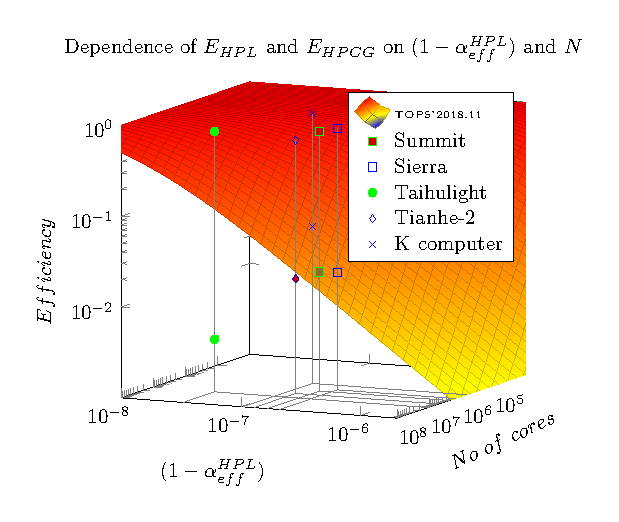
\includegraphics{fig/EffDependence2018LogA.pdf}
		}
	\end{figure}
	%	\pause
	{"The efficency is a feature rather than a bug".}
	
	%	\pause
	{”this decay in performance is not a fault of the
		architecture, but is dictated by the limited parallelism”.\cite{ScalingParallel:1993}}
}


\MEsection[The model]{Amdahl's model}
\MEframe{The model of parallel/sequential operation}
{
	\begin{figure}
		\maxsizebox{\textwidth}{.85\textheight}{
			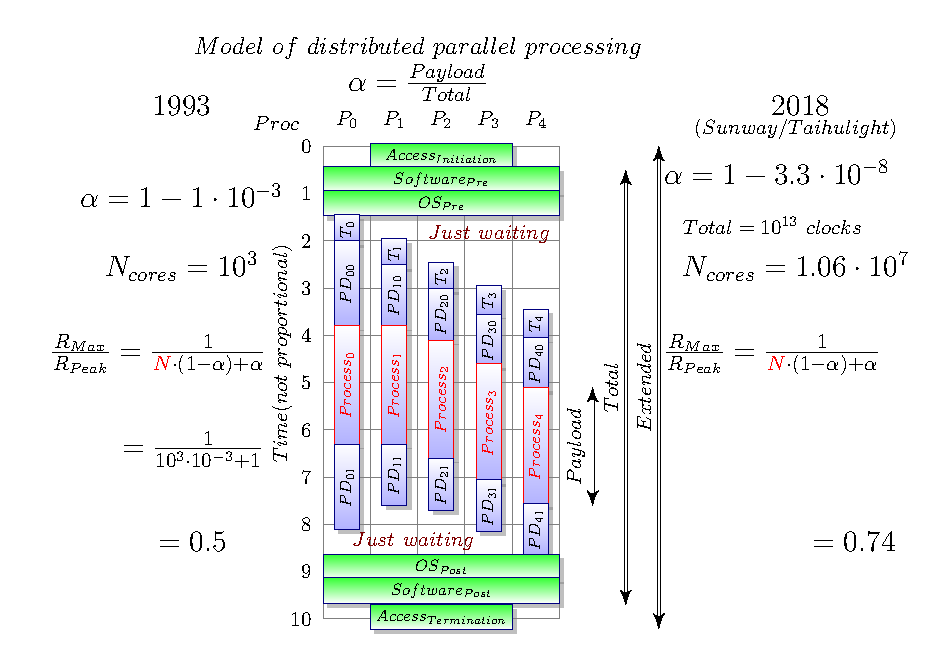
\includegraphics{fig/AmdahlModelAnnotated.pdf}
		}
	\end{figure}
	%	\pause
	\textbf{\textit{SW, \textcolor{red}{HW  and science} contribute to the sequential-only fraction.}}
	
	(The terms of the simple non-technical model need proper interpretation.)
}


%%%% This is the ISC-2020 Frankfurt 2nd tutorial, B2

\MEchapter[History of supercomputing]{History of performance of supercomputing}
\MESetListingFormat[basicstyle={\ttfamily\color{black}\normalsize}]{SystemC}


%\subsubsection{History of performance of supercomputing 45+5'}
%The rigorously verified and detailed database of TOP500 supercomputers
%provides an excellent starting point to draw conclusions.
%It will be demonstrated that the lesson learned: to increase
%the computing performance of the system the "effective parallelization" must also be enhanced, increasing the number of
%processors is not sufficient. It will be demonstrated that
%the "effective parallelization" is a proper merit and enables
%to compare the supercomputers from different ages, technology, manufacturers. The analysis makes clear that 
%the resulting performance stalled: the implementation technology 
%reached its limits.


\MEsection[History of supercomputing]{History of performance of supercomputing}
%%%%%%%%%%%%%%%%%%%%%%%%
\MEframe[shrink]{History of performance of supercomputing}
{
\articleonly{} 

\articleonly{
}	
	The context
}% Lessons

%%% This is the ISC-2020 Frankfurt 2nd tutorial, B3

\MEchapter[Benchmarking]{Benchmarking performance of supercomputing}
\MESetListingFormat[basicstyle={\ttfamily\color{black}\normalsize}]{SystemC}


%\subsubsection{Benchmarking performance of supercomputing 45+5'}
%Based on the contributions, the role of the benchmarking
%method will be discussed. The experience that "supercomputers have
%two different efficiencies" will be interpreted. It will be shown
%that with enhancing the technology of implementation,
%the computation/communication became the major limitation of the supercomputing tasks. The role of the computing workflow (including HPL/HPCG, brain simulation and AI) will be discussed.
%The validity and accuracy of the approach 
%will also be demonstrated. The effect of different technical implementations
%(including GPGPU acceleration, half precision, OpenCAPI bus and interconnection quality) are demonstrated. 

\articleonly{The most obvious 
field to apply our model to is supercomputers. 
Here the number of processors is extremely high and 
-- as will be demonstrated -- all contributions to $(1-\alpha_{eff})$
have been greatly reduced during their very well documented history spanning a quarter of century~\cite{Top500:2016}. Our model is flexible enough to
describe those \gls{HW}/\gls{SW} architectures and also indirectly prove the validity of the principles used in the model.
} 



\MEsection[Workflow type]{The effect of workflow on the performance}
%%%%%%%%%%%%%%%%%%%%%%%%
\MEframe[shrink]{Benchmarking performance of supercomputing}
{
\articleonly{	It is also known since decades that
	"\textit{the inherent communication-to-computation ratio in a
		parallel application is one of the important determinants
		of its performance on any architecture. The higher the
		ratio, the less likely is a machine to provide effective performance on that application}."\cite{ScalingParallel:1993} 
	This observation is demonstrated in Fig.~\ref{fig:AlphaContribBenchmark}. 
	
	The left column of the figure displays different common
	communication intensities (different workflow types).
	The bottom subfigure 
	shows the common case of Artificial Intelligence,
	where some intermediate layers exchange information with
	each other and the rest of the "neurons".
	Notice that here the communication intensity is proportional with $m^2$, the square of the number of "neurons", in the hidden layer.
	
	The middle and bottom subfigures in the left column depict the communication intensity of the two popular supercomputer benchmark programs \gls{HPL} and \gls{HPCG} in the same style. Here the initiating and terminating node is a single core and the "hidden layer" comprises all the rest of the cores. The communication intensity of \gls{HPL} is proportional
	with $N$ (the total number of processing units) and that of	\gls{HPCG} with $h\cdot N$, because $h$ iterations take place. Let us notice that when a supercomputer is utilized for calculation in $AI$
	mode, the $AI$ mode means performance proportional with
	the number of neurons in the hidden layer. If the supercomputer having 1M core is running in \gls{HPL} configuration, and the AI mode system runs on x:1k:1k:y cores, they will have the same performance~\cite{VeghAIperformance:2020}. (The absolute times must not be compared, but their ratio can.)
}
	

	\MEfigure[wide]{fig/AlphaContribBenchmark.pdf}
{The dependence of the payload performance of the different contrinutions and on the workflow type.}
{fig:AlphaContribBenchmark}{}{}

\articleonly{
The right hand column requires more attention. The right-hand scale and the blue line refer to the payload performance. The left hand scale refers to the $\alpha$ contributions of different kinds. For visibility, only the looping (\gls{OS}) contribution and the \gls{SW} (calculation+communication) contributions are shown.
The communication intensity %(and the value of $\alpha$)
is the lowest for the \gls{HPL} case and the highest is for the \gls{AI} case.
Correspondingly, the payload performance is the best for
\gls{HPL} and worst for   \gls{HPL}.

The reason is the different amounts of $\alpha$ contributions. Between subfigures A and B,
the amount (and so the contribution) of the calculation
is increased, mainly because of the need of iteration.
Between subfigures B and C, the communication intensity is increased, leading to orders of magnitude decrease
in the efficiency %(and so in the payload performance)
and also the inflexion point moves tovards much lower
nominal performance values.
% (and so the breakdown can be experienced at much lower number of cores).
}
%
%relative weight of the contributions and the resulting payload performance
}% Lessons

\MEsection[Interconnection]{The effect of interconnection on the performance}

\MEframe[shrink]{The contribution of the interconnection}
{
In a somewhat simplified view, the 
resulting performance can be calculated using the contributions to $\alpha$ as


\begin{equation}
P(N,\alpha) = \frac{N\cdot P_{single}}{\textcolor{red}{N}\cdot \left(1-\textcolor{red}{\alpha_{Net} -\alpha_{Compute}} -\alpha_{Others}    \right)+\approx 1}
\end{equation}

\noindent 
That is, two of the contributions are handled with emphasis. The theory easily provides values for the contributions for
the interconnection and calculation separately.  
Fortunately, the public database TOP500~\cite{Top500:2016}
also provides data measured under conditions greatly similar
to the 'net' contribution.
Of course, the measured data contain the contribution of all components.
However, as will be shown below, in the total contribution those mentioned contributions dominate,
so the measured $\alpha$ can be directly compared with the calculated
$\alpha$, although here only qualitative agreement can be expected.
}


\MEframe[shrink]{The contribution of the interconnection: theory vs measured}
{

	\MEfigure[wide]{fig/InterconnectionVsPerformance.pdf}
{The effect of changing the dominating contribution.
	The left subfigure shows the theoretical estimation,
	the right subfigure the corresponding measured data, as derived from the 
	public database TOP500~\cite{Top500:2016}.}
{fig:InterconnectionVsPerformance}{}{}


\articleonly{
Both the quality of the interconnection and the nominal performance 
are a parametric function of the time, so one can assume on the
theory side that (in a limited time span) the interconnection contribution
was changing as shown in Fig.~\ref{fig:InterconnectionVsPerformance}A.
The other major contribution is assumed to be the calculation\footnote{This time also accessing data ("communicating" is included)} itself.
The benchmark calculation contributions for  \gls{HPL} and \gls{HPCG}
are very different, so the sum of the respective component plus the  
interconnection component are also very different.
Given that at the beginning of the considered time span the 
contribution from the \gls{HPCG} calculation and that of the 
interconnection are in the same order of magnitute, the sum
only changes marginally, i.e. the measured performance changes only marginally.

The case with the \gls{HPL} calculation is drastically different.
Since in this case the contribution from the interconnection is
very much larger than that from the calculation, the sum of these two contributions changes sensitively as the speed of the interconnection
improves. As soon as the contribution from the interconnection
decreases to a value comparable with that of the calculation,
the decrease of the sum slows down considerably,
and the further improvement of the interconnection causes
only marginal decrease in the value of the resulting $\alpha$
(and so only a marginal increase in the payload performance).

The measured data enable to draw the same conclusion,
but one must consider that here multiple parameters may have been
changed. The tendency, however, is surprisingly clear.
Fig.~\ref{fig:InterconnectionVsPerformance}.B is actually a 2.5D diagram: the size of the marks is proportional
with the time passed since the beginning of the considered time period.
A decade ago, the speed of interconnection gave the major contribution
to $\alpha_{total}$; enhancing it drastically in the past few years, increased the efficacy.
At the same time, because of the stalled single-processor performance, the other technology components only changed marginally. The calculation contribution to $\alpha$ from benchmark \gls{HPL}
remained constant in function of the time, so the quick improvement of the interconnection technology resulted 
in a quick decrease of $\alpha_{total}$, and the relative weights of
$\alpha_{Net}$ and $\alpha_{Compute}$ reversed.
\textit{The decrease in value of $(1-\alpha)$ can be considered as 
the result of the decreased contribution from the interconnection.}


However, the total $\alpha$ contribution decreased considerably \textit{only} until $\alpha_{Net}$ reached
the order of magnitude of  $\alpha_{Compute}$. 
This occurred in the first 4-5 years of the time span shown in Fig.~\ref{fig:InterconnectionVsPerformance}.B:
%\ref{fig:compareTheoryMeas}.B: 
the sloping line is due to the 
enhancement of the interconnection.
Then, they changed their role, and the constant contribution due to the calculation started to dominate,
i.e. the total $\alpha$ contribution decreased only marginally.
As soon as the computing contribution took over the dominating role, the total  $\alpha_{total}$
did not decrease any more: all measured data remain above that value of  $\alpha$.
Correspondingly, the payload performance (due to the enhanced interconnection) improved only marginally (and due to factors other than the interconnection).

At this point, as a consequence of that  the dominating contributor changed, it was noticed that the efficacy of the benchmark \gls{HPL} and that of the real-life applications started to differ by up to two orders of magnitude.
At that point was introduced the new benchmark program \gls{HPCG}, since "\textit{\gls{HPCG} is designed to exercise computational and data access patterns that more closely match a different and broad set of important applications%, and to give incentive to computer system designers to invest in capabilities that will have impact on the collective performance of these applications
}"~\cite{HPCG_List:2016}.
Since the major contributor is computing, the different benchmarks contribute differently and since that time
"\textit{supercomputers have two different efficiencies}"~\cite{DifferentBenchmarks:2017}.
Yes, if the dominating $\alpha$ contribution (from the benchmark calculation) is different, then the same computer shows different efficiencies
in function of the calculation it runs.

This enhancement of the interconnection has two important consequences.
First, that the \gls{HPL} benchmarks
at the beginning of the period measured mostly the contribution of the interconnection, after that they measure mostly the contribution due to the \gls{HPL} algorithm; see also below.
Second, since that time, that the interconnection provides less contribution, than the calculation of the benchmark, enhancing the interconnection contributes only to the \textit{dark performance}, rather than to the \textit{payload performance}. 
}
}

\MEsection[Half precision]{The effect of operand length on the performance}


\MEframe[shrink]{Reducing the operand length}
{
Reducing the communication really makes sense, however.
The so called \textit{HPL-AI} benchmark uses Mixed Precision\footnote{Both names are rather inconsequent. On one side, the test itself has not much to do with AI, just uses the operand length common in AI tasks (\gls{HPL}, similarly to \gls{AI}, is a worload type). On the other side, the Mixed Precision is actually Half Precision: it is natural that for multiplication twice as long operands are used temporarily. A different question is that the operations are contracted.}
\cite{MixedPrecisionHPL:2018} rather than Double Precision 
calculations. This enabled to achieve apparently nearly 3 times better
performance gain, that (as correctly stated in the announcement)
"\textit{Achieving a 445 petaflops mixed-precision result on HPL (equivalent to our 148.6 petaflops DP result)}", i.e. the peak DP performance did not change.

\ao{Unfortunately, this achievement has not much to do with
\gls{AI}: it utilizes the data representation commonly used in AI,
but \textit{the achievement comes from accessing less data in memory and using quicker operations on the  shorter data
	rather than reducing the communication intensity}.
For \gls{AI} applications, the limitations remain the same
as described above;
except that when using Mixed Precision,
the efficiency will be better by a factor of 2-3.
}

\ao{
Similarly, exchanging data directly between the processing units~\cite{CooperativeComputing2015} (without using the global memory)
also enhances $\alpha$ (and payload performance)~\cite{TaihulightHPCG:2018},
but it represents a (slightly) different computing paradigm.
Only the two mentioned measured data fall below
the limiting line of $(1-\alpha)$ in Fig.~\ref{fig:InterconnectionVsPerformance}.B. %\ref{fig:compareTheoryMeas}.
}

\ao{A warning sign is that two of the first ten supercomputers
did not provide their \gls{HPCG} performance and other two
used only a small portion of their cores in the \gls{HPCG} benchmarking.
As predicted: "\textit{scaling thus put larger machines at an inherent
	disadvantage}"~\cite{ScalingParallel:1993}.
The reason is Eq.~(\ref{eq:soverk}): using all of their cores
the achievable performance  is not higher (or maybe even lower),
only the power consumption is higher.
The cloud-like supercomputers have definitely a disadvantage
in the \gls{HPCG} competition: the Ethernet-like operation
results in relatively high $(1-\alpha)$ values.}
}

\MEframe[shrink]{The performance of half precision supercomputers}
{

\ao{It is expected that when using half precision (FP16), four times less
data are transferred and manipulated by the system (for Summit, the measured power
consumption data~\cite{MixedPrecisionHPL:2018} underpin the statement), so} it is expected that

$\alpha_{HPL}^{FP64} = 4*\alpha_{HPL}^{FP16}$

\ao{However, the performance is only 3 times higher\footnote{https://blogs.nvidia.com/blog/2019/06/17/hpc-ai-performance-record-summit/}	 than in the case of 
using 64-bit (FP64) operands. Given that the measured payload performance directly reflects the sum of all contributions,
one can assume that the contributions of the two calculations 
plus the rest of the contributions define the $\alpha$ values}
we can conclude from the measurements
that for supercomputer Summit:

$1-\alpha_{HPL}^{FP0}-\alpha_{HPL}^{FP64} = 1.465*10^{-7}$

$1-\alpha_{HPL}^{FP0}-\alpha_{HPL}^{FP16} = 0.488*10^{-7}$


where $\alpha_{HPL}^{FP0}$ is the contribution of all parts independent from the floating manipulation. This quantity is a "zero bitlength floating operation" contribution: the supercomputer makes the stuff needed to perform the \gls{HPL} benchmark,
but the actual FP operations are not performed\footnote{The role of $\alpha_{HPL}^{FP0}$ is akin to execution time of the "empty loop" in programming.}.  From this, 

$\alpha_{HPL}^{FP0} =0.19*10^{-7}$

$\alpha_{HPL}^{FP16} = 0.33*10^{-7}$

$\alpha_{HPL}^{FP64} = 1.3*10^{-7}$

$\alpha_{HPCG}^{FP64} = 208*10^{-7}$

\ao{These data directly underpin that the technology is (almost) perfect:}
the contribution from the benchmark calculation$\alpha_{HPCG}^{FP64}$
is orders of magnitude larger than the contribution from all the rests.
\ao{Recalling that the benchmark program imitates the behavior (as defined
by the resulting $\alpha$) of real-life programs, one can see that} 
\textit{the contribution from the non-computational actors is
about thousand times smaller than the contribution of
the computation+communication itself}.	
}


\MEframe[shrink]{Finally, how many efficiencies do supercomputers have}
{
The ironic remark that \textit{'Perhaps supercomputers should just be required to have written in small letters at the bottom on their shiny cabinets: “Object manipulations in this supercomputer run slower than they appear.”}~\cite{DifferentBenchmarks:2017}' is becoming increasingly relevant.

 \ao{The imposant numbers about performance of the individual components (including single-processor performance and speed of interconnection)
are becoming less relevant when going to the extremes.
Given that the largest $\alpha$ contribution today takes its origin in the
calculation the supercomputer runs, even the best possible benchmark \gls{HPL} dominates the performance measurement.
Enhancing the other contributions, such as interconnection,
result only in marginal enhancement of the performance, i.e.} the 
overwhelming majority of the expenses increases the "dark performance" only. \ao{Because of this,} \textit{there are as many performance values
	as many measurement methods, and actually the benchmarks
	measure how much mathematics/communication the 
	benchmark program does\ao{, rather than the supercomputer architecture
	(provided that all components deliver the technically achievable 
	best parameters)}}. 
}

\MEframe[shrink]{The rooflines of supercomputer performance}
{
\ao{	As it can be concluded from that the many-processor performance
	\textit{has} a maximum, depending on the effective parallelization,
	and that the different workflows result in different effective parallelization,} "\textit{Two Different Top500 Supercomputing Benchmarks Show Two Different Top Supercomputers}"~\cite{DifferentBenchmarks:2017}.
	
	\MEfigure{fig/RooflineBrain.pdf}
{The "rooflines" of supercomputer performance for three different workflows.}
{fig:RooflineBrain}{}{}

\ao{
As discussed above and the theoretical discussion is illustrated in Fig.~\ref{fig:AlphaContribBenchmark},}
the different workflows really contribute differently and they result in different performance gain rooflines~\cite{WilliamsRoofline:2009} \ao{(this expresses the resulting performance without the single processor performance). The measured values are shown in Fig.~\ref{fig:RooflineBrain}
for the commonly used benchmark programs \gls{HPL} and \gls{HPCG}. The third 
roofline level is concluded from the brain simulation measurement~\cite{NeuralNetworkPerformance:2018}, so it is subject of uncertainty.
The roofline values shall be compared to the theoretically derived dependencies demonstrated in Fig.~\ref{fig:AlphaContribBenchmark}.
The fact that the theoretical diagram lines
consider pure and consequently calculated performance values, while the measured values may contain "foreign" contributions (such as the contribution of the interconnection discussed above)
must be kept in mind.

}
}% Lessons


\MEsection[Brain simulation/AI]{The performance of brain simulation and AI}


\MEframe[shrink]{The efficiency of AI solutions}
{
\ao{Today we live in the age of artificial intelligence and machine learning; from small
startups to HW or SW giants everyone wants to build machine intelligence chips, applications,
etc. The task, however, is hard: not only because of the size of the problem:
the technology one can utilize (and the paradigm it is based upon) strongly degrades
the chances to succeed efficiently.} The general principles are of course well known, and the AI systems work more or less as expected for simple tasks, but on large systems they show up miserably small efficacy (extremely high learning times)~\cite{VeghAIperformance:2020}.

\ao{There are, of course, very enhanced solutions, but their technical implementation is "top secret".
Because of this, in this section the "experimental data" refer to the published data of brain simulation~\cite{NeuralNetworkPerformance:2018,SpiNNaker:2013}, where also enough
implementation details are known.
Although the two cases are quantitatively different, the common feature of them is that
as we approach the extremes with the size of
the computing units, the nonlinearity of the scaling becomes more and more obvious.
	}

}

\subsection{Supercomputer efficiency in terms of AI}
MEframe[shrink]{The communication in the AI multi-layer structure}
{
	\MEfigure{fig/AImultilayer.pdf}
{The communication density of the AI workload}
{fig:AImultilayer}{}{}


\ao{Recall the communication density of
	the \gls{AI} workflow, shown in Fig.~\ref{fig:AImultilayer} (formerly shown as subfigure of Fig.~\ref{fig:AlphaContribBenchmark}).
 The life begins in several input channels (rather than one
as in the \gls{HPL} and \gls{HPCG} cases) that would be advantageous.
However, the values must be communicated to \textit{all} nodes in the top hidden layer:
the more input nodes and the more nodes in the hidden layer(s), the many $times$ more 
communication is required for the operation.	
 The same happens also when the
first hidden layer communicates data to the second one; except that here \textit{the square of the number of the nodes} is to be used as a weight factor of communication.

Initially the $n$ input nodes
issue messages, each one $m$ messages (queuing\#1) to the nodes
in the first hidden layer, i.e. altogether $nm$ messages.
If a commonly used shared bus is utilized to transfer 
the messages, these  $nm$ messages must be queued (queuing\#2). 
Also, every single node in the hidden layer
receives (and processes) $m$ input messages (queuing\#3).
Between the hidden layers the same is repeated (maybe several times)
with $mm$ messages, and finally $km$ messages
are sent to the output nodes.
In all cases queuing 3 times.

To make a fair comparison with benchmarks $HPL$ and $HPCG$,
let us assume one input and one output node.
In this case the AI execution time is $O(h\times m^2)$,
provided that $h$ hidden layers are implemented. 
(Here it was assumed that the messaging mechanism
between layers is independent from each other.
It is not so if they share a global bus.
\footnote{\textit{"The idea of using the popular shared bus to implement the communication medium is no longer acceptable, mainly due to its high contention."}~\cite{ReconfigurableAdaptive2016}})

For a numerical example: let us assume that 
in the supercomputers 1M cores are used, and 
in the AI network 1K nodes are present in the hidden layers,
and only one input and output nodes are used.
In that case all execution times are $O(1M)$
(again, the amount of calculation is strongly different,
so the scaling can be compared, but not the execution times).
This communication intensity explains why in Fig.~3 %\ref{fig:rooflines}
the $HPCG$ "roofline" falls
hundreds of times lower than that of the $HPL$: 
the increased communication need strongly decreases
the achievable performance gain.




Notice that} the number \textit{calculation} operations increases with $m$,
while the number of \textit{communication} operations with $m^2$. \ao{In other words:
the more nodes in the hidden layers, the higher is the communication intensity (communication/calculation ratio) and because of this, the lower is the efficiency of the system.
Recall, that since the AI nodes perform simple calculations
compared to the functionality of the supercomputer benchmarks,
the communication/calculation ratio is much higher, 
making the efficacy even worse.

The massively "bursty" nature of the data (the different nodes of the layer
want to use the communication at the same moment) also makes the case harder.
The commonly used global bus is overloaded with messages. 
The possibility for wired point-to-point communication is obviously limited;
but deploying them at least for the inter-layer communication buses can help a lot.




The communication circuits receive the task to send the data to $N$ other nodes.
The calculation and communication are \textit{ab ovo} sequential, and
the communication channel can only transfer one data value at a time.
What is worse,}
 bus arbitration, addressing, latency, etc. prolong the transfer time (and in his way decreases efficacy of the system).

}


\subsection{Accelerating supercomputer using GPGPU}
\MEframe[shrink]{GPGPU}
{
%	\MEfigure{fig/AImultilayer.pdf}
%	{The communication density of the AI workload}
%	{fig:AImultilayer}{}{}
%	
%\MEfigure{fig/CommunicationCollapse.pdf}
%{Demonstrating the communicational collapse at large workloads}
%{fig:CommunicationCollapse}{\protect{\cite{CommunicationCollapse:2018}}}{}
}

%\subsection{Supercomputer efficiency in terms of AI}
%\MEframe[shrink]{The communication in the AI multi-layer structure}
%{
%	\MEfigure{fig/AImultilayer.pdf}
%	{The communication density of the AI workload}
%	{fig:AImultilayer}{}{}

%%%% This is the ISC-2020 Frankfurt 2nd tutorial, B4

\MEchapter[Modern computing]{Modern science and modern computing}
\MESetListingFormat[basicstyle={\ttfamily\color{black}\normalsize}]{SystemC}


%\subsubsection{Modern science and modern computing 45+5'}
%The parallel with the modern science is completed:
%it will be shown that under extreme conditions the "quantal nature
%of time" manifests and "communicational collapse" occurs,
%caussing demonstrative failures of supercomputers and brain simulators.
%Also, that measuring the performance of a many-many processor
%parallelized sequential computing system casuses a drastic  
%change in the state of the supercomputer, in a completely analogous 
%way with measuring the state of a quantum system.
%Based on the investigations presented above, the short-time 
%future of supercomputing will be predicted. Given that the
%major contributor to the non-parallelizable portion of the task
%is the computation/communication itself, the further technical enhancement, without changing the principle of computation is "mission impossible": only increase the "dark performance" of the computing systems with extreme size. The tutorial will convincingly demonstrate
%the need for a new computing paradigm, and also a possible way out will be sketched. 



\MEframe{Analogy with the relativistic speed addition}
{%
%	\maxsizebox{\textwidth}{!}
	{
		\begin{figure*}
		\begin{tabular}{cc}
			\only<1->
			{\maxsizebox{.5\textwidth}{!}
				{
					
					
					\def\LightSpeed{3.e8}	% m/s
					\def\Gravity{10.}		%m/s^2
					\def\Speed{x*\Gravity}
					\def\RelSpeedFactor{\Speed/(\LightSpeed/\Density)}
					\def\RelSpeed{\Speed/sqrt(1+\RelSpeedFactor*\RelSpeedFactor)}
					
					\def\RelSpeedFactorB{\Speed/(\LightSpeed/\Density/2)}
					\def\RelSpeedB{\Speed/sqrt(1+\RelSpeedFactorB*\RelSpeedFactorB)}
					
					\def\OneDay{86400}
					
					\begin{tikzpicture}%[scale=1.5]
					\begin{axis}[
					%  axis y line*=left,
					title={\huge Relativistic speed of body accelerated by 'g'},
					width=\textwidth,
					%	title style={at={(0.5,1.05)},anchor=north},
					%	title = {Relativistic speed of body accelerated by 'g'}, 
					xlabel=\huge $time(s)$,
					ylabel=\huge $speed (m/s)$,
					ymin=1e6, ymax=5e8,
					xmin=\OneDay, xmax=5e8,
					xmode=log,
					log basis x=10,
					ymode=log,
					log basis y=10,
					legend style={
						cells={anchor=west},
						legend pos={north west},
					},
					]
					\def\Density{1.}
					
					\addlegendentry{$v(t),~n=1$}
					\addplot[samples=501,domain=\OneDay:1e9,webgreen]
					{\RelSpeed} ;\label{plot_loo}\OneDay
					
					\def\Density{2.5}
					\addplot[samples=501,domain=\OneDay:1e9,webred]
					{\RelSpeed} ;\label{plot_loo}
					\addlegendentry{$v(t),~n=2.5$}
					
					\def\Density{5.}
					\addplot[samples=501,domain=\OneDay:1e9,webred]
					{\RelSpeed} ;\label{plot_loo}
					\addlegendentry{$v(t),~n=5$}
					
					\end{axis}
					
					
					\end{tikzpicture}
				}
				
			}&
			\only<2->
			{
				\maxsizebox{.5\textwidth}{!}
				{
					
					\def\alpha{(1-\beta)}
					
					\def\N{(x/0.0000001)}
					%	\def\PayloadPerformance{x/(\N*(1.-\alpha)+ \alpha)}%(\N*(1-\alpha)+\alpha)}
					\def\PayloadPerformance{x/(\alpha+100000000*x*\beta)}
					\def\betaN{1e-10}
					\def\betaA{1e-8}
					\def\betaB{1e-7}
					\def\betaC{1e-6}
					\def\betaD{1e-5}
					
					\begin{tikzpicture}%[scale=1.5]
					\begin{axis}[
					%  axis y line*=left,
					title={\huge Payload performances of N cores @100GFlops},
					width=\textwidth,
					%	title style={at={(0.5,1.05)},anchor=north},
					%	title = {Relativistic speed of body accelerated by 'g'}, 
					xlabel=\huge Nominal performance (EFlops),
					ylabel=\huge Payload performance (EFlops),
					ymin=1e-4, ymax=2,
					xmin=1e-4, xmax=2,
					xmode=log,
					log basis x=10,
					ymode=log,
					log basis y=10,
					legend style={
						cells={anchor=west},
						legend pos={north west},
					},
					]
					\def\beta{\betaN}
					
					\addlegendentry{1-$alpha=\betaN$}
					\addplot[samples=501,domain=1e-4:2,webred]
					{\PayloadPerformance} ;%\label{plot_0}
					\def\beta{\betaA}
					
					\addlegendentry{1-$alpha=\betaA$}
					\addplot[samples=501,domain=1e-4:2,webgreen]
					{\PayloadPerformance} ;%\label{plot_0}
					
					\def\beta{\betaB}
					
					\addlegendentry{1-$alpha=\betaB$}
					\addplot[samples=501,domain=1e-4:2,webgreen]
					{\PayloadPerformance} ;%\label{plot_0}
					
					\def\beta{\betaC}
					
					\addlegendentry{1-$alpha=\betaC$}
					\addplot[samples=501,domain=1e-4:2,webgreen]
					{\PayloadPerformance} ;%\label{plot_0}
					
					\def\beta{\betaD}
					
					\addlegendentry{1-$alpha=\betaD$}
					\addplot[samples=501,domain=1e-4:2,webblue]
					{\PayloadPerformance} ;%\label{plot_0}
					\end{axis}
					
					
					\end{tikzpicture}
					
			}}\\
		\end{tabular}
	\caption{A body accelerated by a constant gravitational force cannot exceed the speed of light.
The performance of a parallelized sequential computing system 
		cannot exceed its specific 'speed of light'.
				The performance is sensitive to the amount of computation (including data length) and communication. Science is \textbf{not} limiting below EPlops performance.
			\label{fig:LingtSpeedVsPerformance}
		}
	\end{figure*}
}
}

\MEframe{The resulting performance and its contributions}
{%
  Recall that in general:
  
			\Large $ P(N) = \frac{N\cdot P_{single}}{\boxed{\textcolor{red}{N\cdot \left(1-\alpha\right)+\alpha}}}$
			

  This enables (at least theoretically) to consider 
  the contributions separately, and if some contrution is dominant,
  to see its effect in measurement data:  
   	
   	\maxsizebox{\columnwidth}{!}
   	{
			\Large $ P(N) = \frac{N\cdot P_{single}}{\boxed{\textcolor{red}{N}\cdot \left(1-\alpha_{Science}  
						\textcolor{red}{-\alpha_{Net} -\alpha_{Compute}} -\alpha_{Others}    \right)+\approx 1}}$
					}
	
}


\MEsection{The final cut}

\MEframe{The effect of calculations/measuring}
{%
	\maxsizebox{\textwidth}{!}
	{
		\begin{tabular}{p{.5\textwidth}p{.5\textwidth}}
			\only<1->
			{
				
				\maxsizebox{.5\textwidth}{!}
				{
					
					\def\alpha{(1-\beta)}
					
					\def\N{(x/0.0000001)}
					%	\def\PayloadPerformance{x/(\N*(1.-\alpha)+ \alpha)}%(\N*(1-\alpha)+\alpha)}
					\def\PayloadPerformance{x/(\alpha+15000000*x*\beta)}
					\def\betaN{1e-10}
					\def\betaA{0.19 e-7}
					\def\betaB{1.465 e-7}
					\def\betaC{0.488 e-7}
					\def\betaD{208 e-7}
					
					\begin{tikzpicture}%[scale=1.5]
					\begin{axis}[
					%  axis y line*=left,
					title={\huge Payload performances @Summit},
					width=\textwidth,
					%	title style={at={(0.5,1.05)},anchor=north},
					%	title = {Relativistic speed of body accelerated by 'g'}, 
					xlabel=\huge Nominal performance (EFlops),
					ylabel=\huge Payload performance (EFlops),
					ymin=1e-4, ymax=2,
					xmin=1e-4, xmax=2,
					xmode=log,
					log basis x=10,
					ymode=log,
					log basis y=10,
					legend style={
						cells={anchor=west},
						legend pos={north west},
					},
					]
					\def\beta{\betaD}
					
					\addlegendentry{1-$alpha=HPCG-FP64$}
					\addplot[thick,samples=501,domain=1e-4:2,webblue]
					{\PayloadPerformance} ;%\label{plot_0}
					
					\def\beta{\betaC}
					\addlegendentry{1-$alpha=HPL-FP64 $}
					\addplot[thick,samples=501,domain=1e-4:2,webgreen]
					{\PayloadPerformance} ;%\label{plot_0}
					
					\def\beta{\betaB}
					
					\addlegendentry{1-$alpha=HPL-FP16$}
					\addplot[thick,samples=501,domain=1e-4:2,webgreen]
					{\PayloadPerformance} ;%\label{plot_0}
					
					\def\beta{\betaA}
					
					\addlegendentry{1-$alpha=HPL-FP0$}
					\addplot[thick,samples=501,domain=1e-4:2,orange]
					{\PayloadPerformance} ;%\label{plot_0}
					
					\def\beta{\betaN}
					
					\addlegendentry{1-$alpha=Science$}
					\addplot[thick,samples=501,domain=1e-4:2,webred]
					{\PayloadPerformance} ;%\label{plot_0}
					
					\addplot[only marks,  mark=o,  mark size=5, thick] plot coordinates {
						(0.2008,0.148) %Summit @HPL-FP64
						%	(0.2008,0.445) %Summit @HPL-FP16
						(0.602,0.445) %Summit @HPL-FP16
						(0.2008,0.00293) %Summit @HPCG-FP64
					};
					
					\end{axis}
					
					
					\end{tikzpicture}
					
				}
			}
			&
			\only<2->
			{
				\maxsizebox{.5\textwidth}{!}
				{
					
					\def\alpha{(1-\beta)}
					
					\def\N{(x/0.0000001)}
					%	\def\PayloadPerformance{x/(\N*(1.-\alpha)+ \alpha)}%(\N*(1-\alpha)+\alpha)}
					\def\PayloadPerformance{x/(\alpha+15000000*x*\beta)}
					\def\betaN{1e-10}
					\def\betaA{0.19 e-7}
					\def\betaB{1.465 e-7}
					\def\betaC{0.488 e-7}
					\def\betaD{208 e-7}
					
					\begin{tikzpicture}%[scale=1.5]
					\begin{axis}[
					%  axis y line*=left,
					title={\huge Payload performances @Exascale},
					width=\textwidth,
					%	title style={at={(0.5,1.05)},anchor=north},
					%	title = {Relativistic speed of body accelerated by 'g'}, 
					xlabel=\huge Nominal performance (EFlops),
					ylabel=\huge Payload performance (EFlops),
					ymin=1e-4, ymax=1000,
					xmin=1e-4, xmax=5000,
					xmode=log,
					log basis x=10,
					ymode=log,
					log basis y=10,
					legend style={
						cells={anchor=west},
						legend pos={north west},
					},
					]
					\def\beta{\betaD}
					
					\addlegendentry{1-$alpha=HPCG-FP64$}
					\addplot[thick,samples=501,domain=1e-4:10000,webblue]
					{\PayloadPerformance} ;%\label{plot_0}
					
					\def\beta{\betaC}
					\addlegendentry{1-$alpha=HPL-FP64 $}
					\addplot[thick,samples=501,domain=1e-4:10000,webgreen]
					{\PayloadPerformance} ;%\label{plot_0}
					
					\def\beta{\betaB}
					
					\addlegendentry{1-$alpha=HPL-FP16$}
					\addplot[thick,samples=501,domain=1e-4:10000,webgreen]
					{\PayloadPerformance} ;%\label{plot_0}
					
					\def\beta{\betaA}
					
					\addlegendentry{1-$alpha=HPL-FP0$}
					\addplot[thick,samples=501,domain=1e-4:10000,orange]
					{\PayloadPerformance} ;%\label{plot_0}
					
					\def\beta{\betaN}
					
					\addlegendentry{1-$alpha=Science$}
					\addplot[thick,samples=501,domain=1e-4:10000,webred]
					{\PayloadPerformance} ;%\label{plot_0}
					
					\addplot[only marks,  mark=o,  mark size=5, thick] plot coordinates {
						(0.2008,0.148) %Summit @HPL-FP64
						%	(0.2008,0.445) %Summit @HPL-FP16
						(0.602,0.445) %Summit @HPL-FP16
						(0.2008,0.00293) %Summit @HPCG-FP64
					};
					
					
					\end{axis}
					
					
					\end{tikzpicture}
					
				}
			}
		\end{tabular}
	}
	\only<1>{A supercomputer has different limiting factors.
		
	}
	\only<2->{
		At exascale, the science (the speed of light) becomes a limiting factor.
		
		The performance of the computing system behaves as a quantal system:
		as soon as you start to measure the performance, the contribution of the measuring device (benchmark program) starts to dominate
	}
	
}


\subsection{The quantal nature of time}

\MEframe[shrink]{The brain simulation and the quantal nature of time}
{
	
	The processor-based brain simulation provides an
	"experimental evidence"~\cite{VeghBrainAmdahl:2019} that the time in computing shows quantal behavior, analogously with the energy in physics. When simulating neurons using processors,
	the ratio of the simulated (biological) time and the processor time used to simulate the biological effect may considerably differ, so to avoid working with "signals from the future", periodic synchronization is required that introduces a special "biological clock cycle".
	The role of this clock period is the same as that of the clock signal in the clocked digital electronics: what happens in this period, it happens "at the same time"\footnote{This periodic synchronization will be a limiting factor in large-scale utilization of processor-based artificial neural chips~\cite{IntelLoihi:2018}, although thanks to the cca. thousand times higher "single-processor performance", only when approaching the computing capacity of (part of) the brain.}.
	
	The brain simulation (and in somewhat smaller scale: artificial neural computing) requires intensive data exchange between the parallel threads:
	the neurons are expected to tell the result of their neural calculations periodically to thousands of fellow neurons.
	The commonly used $1~ms$ "grid time" is,
	however, $10^6$ times longer than the
	$1~ns$ clock cycle common in the digital electronics~\cite{NeuralNetworkPerformance:2018}.
	Correspondingly, its influence on the performance is noticeable.
	Figure~\ref{fig:AlphaContribBenchmark}
	.C demonstrates what happens if the clock cycle is 5000 times longer than in Figure~\ref{fig:AlphaContribBenchmark}
	.B:
	it causes a drastic decrease in the achievable performance and strongly shifts the performance breakdown toward lower nominal performance values.
	As shown, the "quantal nature of time" in computing
	changes the behavior of the performance drastically.
	
	
	
	In addition, the thousands times more communication contributes considerably to the non-payload sequential-only fraction,
	so it degrades further the efficacy of the computing system.  What is worse, they are expected to send their messages at the end of the grid time period, causing a huge burst of messages.
}

\subsection{The communicational collapse}
\MEframe[shrink]{The communicational collapse}
{
	
	\MEfigure{fig/CommunicationCollapse.pdf}
	{Demonstrating the communicational collapse at large workloads}
	{fig:CommunicationCollapse}{\protect{\cite{CommunicationCollapse:2018}}}{}
	
	
	
	
	\ao{
		Not only the achievable performance is by orders of magnitude lower,
		but also the "communicational collapse"~\cite{CommunicationCollapse:2018} (see also~\cite{ScalingParallel:1993}) occurs at orders of
		magnitude lower nominal performance. 
		This is the reason why less than one percent of the planned capacity
		can be achieved even by the custom built large scale ANN simulators~\cite{SpiNNaker:2013}.
		Similarly, the SW and HW based simulators show up the same limitation~\cite{NeuralNetworkPerformance:2018,VeghBrainAmdahl:2019}.
		This is why only a few dozens of thousands of neurons can be simulated on processor-based brain simulators (including both the many-thread software simulators and the purpose-built brain simulator)~\cite{NeuralNetworkPerformance:2018}.
		The memory of extremely large supercomputers can be populated with objects simulating neurons~\cite{SpikingPetascale2014}, but as soon as they need to communicate,
		the task collapses as predicted in Figs.~\ref{fig:AlphaContribBenchmark} and~\ref{fig:CommunicationCollapse}. This is indirectly underpinned~\cite{NeuralScaling2017} by that the different handling
		of the threads changes the efficacy sensitively and that the time required for more detailed simulation increases non-linearly~\cite{NeuralNetworkPerformance:2018,VeghBrainAmdahl:2019}.
	}
}


\MEsection{A possible way out}
\MEframe{The Explicitly Many-Processor Approach}
{% 
	We really need a \textit{modern computing paradigm}. Major items:
	\begin{itemize}
		\item the processing capability is one of the resources 
		\item not the \textbf{same} processor must do 
		every single operation
		\item flexibly adapt the architecture to the task
		\item communication with other processing units is a native feature
		\item the hardware and software exist only together
		\item the tasks are broken into appropriately sized and logically interconnected fragments
		\item the code fragments are to be executed in parallel, provided both data dependence and hardware availability enables it
		\item the principle of locality is applied to memory handling at hardware level, through direct wiring and hierarchic buses
	\end{itemize}
}


%%%% This is the WrapUp of the ISC-2020 Frankfurt tutorials 

\MEchapter[WrapUp]{WrapUp}
\MESetListingFormat[basicstyle={\ttfamily\color{black}\normalsize}]{SystemC}

\MEsection[WrapUp]{WrapUp}
%%%%%%%%%%%%%%%%%%%%%%%%
\MEframe[shrink]{WrapUp}
{
\articleonly{} 

\articleonly{
}	
	The context
}% Lessons


\MEframe{Strategy, investment and political will - 2016}
{
	\MEquote{	
		the largest HPC hardware systems today
		contain more than 1 million cores, and exascale
		supercomputers with tens or hundreds of millions
		of cores will begin to arrive during the period
		2020-2022 " and "With a differentiated strategy
		and sufficient investment and political will,
		Europe can be a global player in HPC.}
	{Europe Union’s Action plan, 2016)}
}	

\MEframe{Results/continuation} 
{
	\begin{itemize}
		\item the present computing paradigm is not usable for the present non-computing applications
		\item the problem must be faced: no more chances to circumvent it 
		\item the \textit{modern computing paradigm} 		successfully explains unexpected phenomena
		and \textit{predicts more phenomena}
		\item based on it, \textit{implementation can be changed
			to enhance computing}
	\end{itemize}
	\vspace{.5 cm}	\pause
	\textit{
		This work is supported by the National
		Research, Development and Innovation Fund of
		Hungary, under  K funding scheme Projects no. 125547 and 132683, as well as ERC-ECAS support of project 861938 is acknowledged	}
}


 \bibliographystyle{IEEEtran}
\bibliography{../../CommonBibliography,%
	../../CommonPrivateBibliography%
}
	\MEbackmatter
\end{document}

%egregious = extremely bad in a way that is very noticeable
%	\input{src/Overview}
%	\part{Basic tutorial}
%  	\MEchapter[Single Processor Approach]{SPA: Around single-processor performance}
%    	\MEsection[Single-Processor Performance]{The Single-Processor Approach}
%    	\MEsection[Limitations of SPA]{Limitations of single-processor performance (Moore's Law)}
%    	\MEsection [Measure performance]{How to measure single-processor performance}
% 		\MEsection[Sequential and parallel] {What is sequential, parallel and parallelized sequential}
%		\MEsection[What is parallel]{What is parallel and concurrent and parallelized sequential performance special in}
%		
% 	\MEchapter[Limitations of parallelization]{Limitations of parallelized sequential performance (Amdahl's Law)}
%		\MEsection[Limitations]{Limitations of parallelized performance: Amdahl's Law}
%      	\MEsection[Amdahl's Law]{Amdahl's definition and model}	
%%		
\MEchapter[A model]{A generalized model of parallelized sequential operation}


\MEsection[Lessons]{Amdahl's model, detailed}
%%%%%%%%%%%%%%%%%%%%%%%%
\MEframe[shrink]{Amdahl's model, annotated}
{
\articleonly{
	The huge variety of the \gls{HW}/\gls{SW} solutions
	with their partly parallel, overlapping, pipelined, networked, predited, retired, etc. solutions make practically impossible to set up a general model of the parallelized sequential operation.
	\index{Model!parallelized sequental operation}
	\index{parallelized sequental operation!Model}
}
\MEfigure[wide]{fig/AmdahlModelAnnotated}{The annotated general model of Amdahl}{fig:ISCsurveyAmdahlAnnotated}
{\protect{\cite{VeghModernParadigm:2019}}, 2019}{}


The figure shows the global contributions of a 
parallelized sequential operation, according to Amdahl's model}


	- \MEsection[Deriving the effective parallelization] {Deriving the effective parallelization}
	- \MEsection[The contributors]{The contributors to the effective parallelization }
	- \MEsection[The limiting contributions] {Limiting effect of the contributions}

%		\MEsection[The effective parallelization]{The role of the effective parallelization }
%		\MEsection[The "dark performance"]{The "dark performance" or the "supercomputer efficiency"}
%   		\MEsection[Amdahl's abusing]{Abusing and misinterpreteting Amdahl's Law}	
%
%		
%  	\MEchapter[Parallel performance]{The performance of parallelization}
%		\MEsection[What is wrong with SPA]{What is wrong with parallelization in SPA}
%		\MEsection[Many-core parallelization]{Many-core parallelization}
%		\MEsection[What kinds of performances exist]{What kinds of performances exist}
%		\MEsection[SW parallelization]{SW parallelization}
%		\MEsection[Parallelization in the cloud]{Parallelization in the cloud}
%	
%  	\MEchapter[Modern computing I]{Analogy with the sciences: counter-intuitive, shocking but true}
%	  	\MEsection[Relativity and computing]{Relativity and computing performance}
%	  	\MEsection[The measurement paradox]{The measurement paradox}
%
%	\part{Performance of HPC}
%  	\MEchapter[High performance] {How to achieve high performance}
%  		\MEsection[Optimization]{Single-thread vs many-processor optimization}
% 		\MEsection[Supercomputing performance]{The performance of supercomputing}
%		\MEsection[The contributions]{The contribution to effective parallelization}
%		\MEsection[The limiting factors]{The limiting factors}
%		
%  	\MEchapter[Benchmark performance]{What actually the benchmark programs measure}
%		\MEsection[Performance of supercomputing]{The performance limitations of supercomputing}
%		\MEsection[Benchmarking]{What actually the benchmark programs measure}
%		\MEsection[Half precision]{Reducing Operand length}
%		\MEsection[Workflow]{The role of workflow mode}
%		\MEsection[Why some supercomputers failed]{Why some supercomputers failed (and why more will fail)}
%		
%  	\MEchapter[Modern computing II]{Analogy with the sciences: counter-intuitive, shocking but true}
%		\MEsection[Collapse]{Gravitational and communicational collapse}
%		\MEsection[The quantal nature]{The quantal nature of (computing) time}
%		\MEsection[Interaction and communication]{Collective behavior}
%
%	\MEchapter[The exa-scale race]{What required to enter the exa-scale race}
%		
%		\MEsection[The "dark performance"]{How to increase the "dark performance"}
%  		\MEsection[The Explicitly Many-Processor Approach]{EMPA: a posible way out}
%	
%\section{Detailed description of the tutorial content (3 pages maximum)}
